\apendice{Documentación de Usuario}
\label{apendice:manual_usuario}

\section{Introducción}
\label{sec:manual_intro}
Este manual proporciona una guía detallada para el despliegue y uso de la infraestructura de procesamiento de vídeo desarrollada en este TFG. El objetivo es ofrecer al usuario técnico (en adelante, el Administrador) todos los pasos necesarios para poner en marcha el sistema completo.

La infraestructura consta de dos sistemas modulares que se despliegan de forma independiente pero que trabajan de manera conjunta: un servidor de captura de vídeo (Jitsi) y un pipeline de procesamiento de datos (Kafka y Spark).

\section{Requisitos Previos del Sistema}
\label{sec:manual_requisitos}
Antes de comenzar, es fundamental asegurar que la máquina anfitriona (\textit{host}) cumple con los siguientes requisitos.

\subsection{Requisitos de \textit{Hardware}}
\begin{itemize}
    \item \textbf{CPU:} Se recomienda un procesador de 4 o más núcleos con soporte para virtualización (VT-x/AMD-V) habilitado en la BIOS/UEFI.
    \item \textbf{Memoria RAM:} Debido a la cantidad de servicios, se recomienda un mínimo de \textbf{16 GB de RAM}.
    \item \textbf{Almacenamiento:} Mínimo de 50 GB de espacio libre en disco.
\end{itemize}

\subsection{Requisitos de Software del Sistema Anfitrión (\textit{Host})}
\begin{itemize}
    \item \textbf{Sistema Operativo:} Se requiere una distribución de Linux. Todo el desarrollo y validación se ha realizado sobre \textbf{Debian 12 "Bookworm"}.
    \item \textbf{Software Base:} Es necesario tener instalados los siguientes paquetes a través del gestor de paquetes \texttt{apt}:
        \begin{itemize}
            \item \texttt{git}: para la clonación de los repositorios.
            \item \texttt{docker.io}: motor de contenedores Docker.
            \item \texttt{docker-compose-v2}: herramienta de orquestación (\textit{plugin} de Docker).
            \item \texttt{curl} y \texttt{openssl}: herramientas de diagnóstico de red.
        \end{itemize}
    \item \textbf{Módulo del Kernel para Jibri:} Para que el servicio de grabación Jibri funcione correctamente y no genere vídeos con pantalla en negro, es \textbf{crítico} instalar el siguiente módulo del kernel que crea un dispositivo de vídeo virtual:
    \begin{verbatim}
sudo apt update
sudo apt install v4l2loopback-dkms
    \end{verbatim}
    Tras la instalación, se recomienda reiniciar el sistema anfitrión.
\end{itemize}

\subsection{Requisitos de Red (para Jitsi)}
Para que el servidor Jitsi sea accesible desde internet y pueda obtener un certificado SSL/TLS válido, se necesita:
\begin{itemize}
    \item Un \textbf{nombre de dominio público}. Para este proyecto se utilizó un dominio gratuito de \textbf{DuckDNS}.
    \item Acceso al \textbf{\textit{router}} para configurar la \textbf{re-dirección de puertos} (\textit{Port Forwarding}) de los puertos TCP 80, TCP 443 y UDP 10000 hacia la IP privada de la máquina anfitriona.
\end{itemize}
(Recomendado) Asignar una dirección IP local estática a la máquina anfitriona en la configuración del \textit{router} (Reserva de DHCP). Esto asegura que la re-dirección de puertos no falle si la IP local del servidor cambia.

\begin{figure}[H]
    \centering
    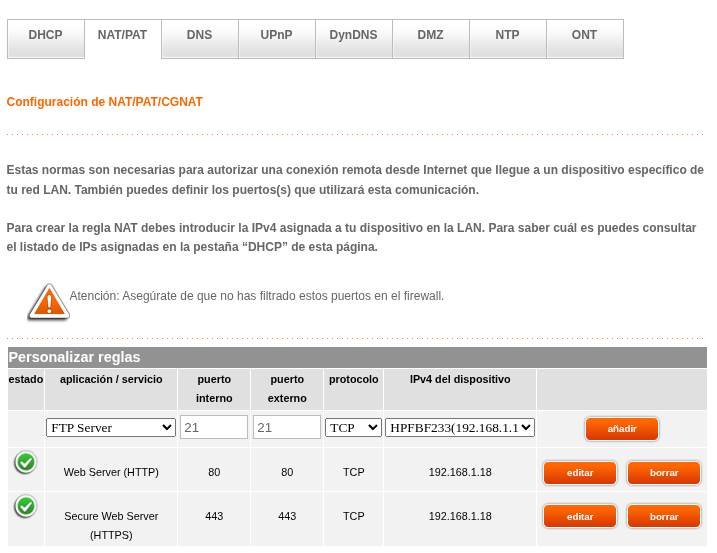
\includegraphics[width=0.9\textwidth]{img/routerconfig.png}
    \caption{Captura de configuración correcta personalizada puertos.}
    \label{fig:puertos_confi_anexoe}
\end{figure}
\begin{figure}[H]
    \centering
    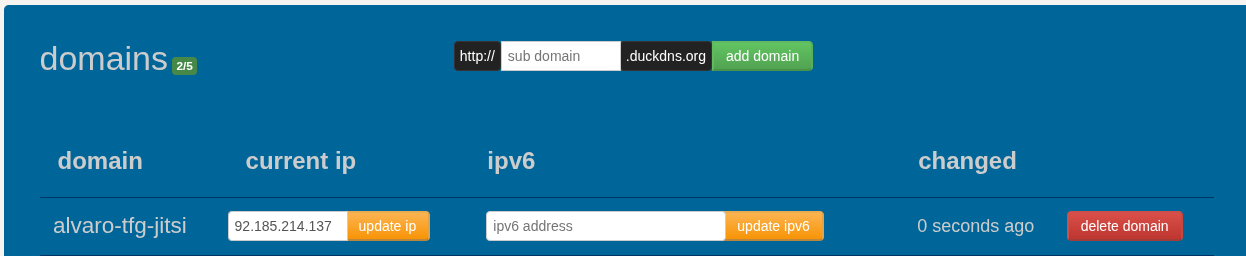
\includegraphics[width=0.9\textwidth]{img/duckdns.png}
    \caption{Captura de servicio Duckdns configurado.}
    \label{fig:duckdns_anexoe}
\end{figure}

\section{Instalación del Sistema}
\label{sec:manual_instalacion}
La instalación se divide en dos fases: el despliegue del servidor Jitsi y, posteriormente, el despliegue del pipeline de procesamiento.

\subsection{Fase 1: Despliegue del Servidor de Captura (Jitsi)}
\begin{enumerate}
    \item \textbf{Clonar el repositorio oficial de \texttt{docker-jitsi-meet}:}
    \begin{verbatim}
git clone https://github.com/jitsi/docker-jitsi-meet.git
cd docker-jitsi-meet
    \end{verbatim}

    \item \textbf{Copiar y configurar el fichero de entorno:} Se debe copiar el fichero de ejemplo y editarlo para ajustar los parámetros a nuestro entorno.
    \begin{verbatim}
cp env.example .env
nano .env
    \end{verbatim}
    Dentro del fichero \texttt{.env}, es crucial configurar las siguientes variables:
    \begin{itemize}
        \item \texttt{PUBLIC\_URL}: El dominio público que se utilizará \\(ej. \texttt{https://mi-tfg.duckdns.org}).
        \item \texttt{LETSENCRYPT\_DOMAIN}: El mismo nombre de dominio.
        \item \texttt{LETSENCRYPT\_EMAIL}: Un correo electrónico para la gestión de los certificados Let's Encrypt.
        \item Habilitar Jibri y la grabación: \texttt{ENABLE\_RECORDING=1},\\ \texttt{ENABLE\_LIVESTREAMING=0}.
    \end{itemize}

    \item \textbf{Generar contraseñas:} Se ejecuta el \textit{script} proporcionado para generar todas las contraseñas internas de los servicios.
    \begin{verbatim}
./gen-passwords.sh
    \end{verbatim}

    \item \textbf{Crear directorios de configuración persistente:}
    \begin{verbatim}
mkdir -p ~/.jitsi-meet-cfg/{web/letsencrypt,transcripts,prosody \ 
/config,prosody/prosody-plugins-custom,jicofo,jvb,jigasi,jibri}
    \end{verbatim}
    \textbf{Nota Importante sobre la Configuración Web:} Es crucial verificar que dentro del directorio ~/.jitsi-meet-cfg/web/ no se cree accidentalmente una carpeta/archivo llamada "\textit{custom.config.js}". Si fuera necesario modificar la configuración del cliente, se deberá crear un fichero de texto con ese nombre.

    \item \textbf{Levantar los servicios de Jitsi:} Se utiliza el siguiente comando para iniciar todos los contenedores, incluyendo Jibri.
    \begin{verbatim}
docker compose -f docker-compose.yml -f jibri.yml up -d
    \end{verbatim}
\end{enumerate}

\subsection{Fase 2: Despliegue del Pipeline de Procesamiento}
\begin{enumerate}
    \item \textbf{Clonar el repositorio del TFG:} En una carpeta diferente, se clona el repositorio principal del proyecto.
    \begin{verbatim}
git clone https://github.com/alvaromarquez1002/ \ 
TFG-SISTEMA-PROCESAMIENTO-VIDEO.git
cd TFG-SISTEMA-PROCESAMIENTO-VIDEO/src
    \end{verbatim}
    
    \item \textbf{Configurar el volumen de datos:} Es importante verificar que en el fichero \texttt{docker-compose.yml} de esta carpeta, el volumen del servicio \texttt{python-processor} esté correctamente mapeado al directorio donde Jibri guarda las grabaciones \\ (por defecto, \texttt{\textasciitilde{}/.jitsi-meet-cfg/jibri/recordings}).
    (Opcional) Para realizar pruebas de desarrollo sin depender de Jitsi, se puede comentar la línea del volumen de Jibri en el fichero docker-compose.yml y activar una línea alternativa como - ./data:/app/data para usar vídeos de prueba locales.

    \item \textbf{Levantar los servicios del pipeline:} Desde la carpeta \texttt{/src}, se ejecuta el siguiente comando. La opción \texttt{--build} asegura que la imagen Docker del procesador se construya con el código más reciente.
    \begin{verbatim}
docker compose up --build -d
    \end{verbatim}
\end{enumerate}

\section{Manual de Uso}
\label{sec:manual_uso}
Una vez desplegados ambos sistemas, el flujo de trabajo para capturar y procesar una sesión es el siguiente.

\subsection{Realizar una Grabación con Jitsi}
\begin{enumerate}
    \item \textbf{Acceder a la conferencia:} El Terapeuta y el Paciente acceden a la URL del servidor Jitsi (ej. \texttt{https://mi-tfg.duckdns.org}) desde sus navegadores web.

    \begin{figure}[H]
    \centering
    
\includegraphics[height=0.6\textheight]{img/entrarreunion.jpg}
    \caption{Pantalla de inicio de Jitsi Meet donde el usuario inicia la conferencia.}
    \label{fig:manual_entrar_reunion}
    \end{figure}
    
    \item \textbf{Iniciar la grabación:} Una vez en la sala, el Terapeuta hace clic en el botón de "Más acciones" (tres puntos verticales) y selecciona la opción "Iniciar grabación". Se le pedirá confirmación para iniciar la sesión.
    \begin{figure}[H]
    \centering
    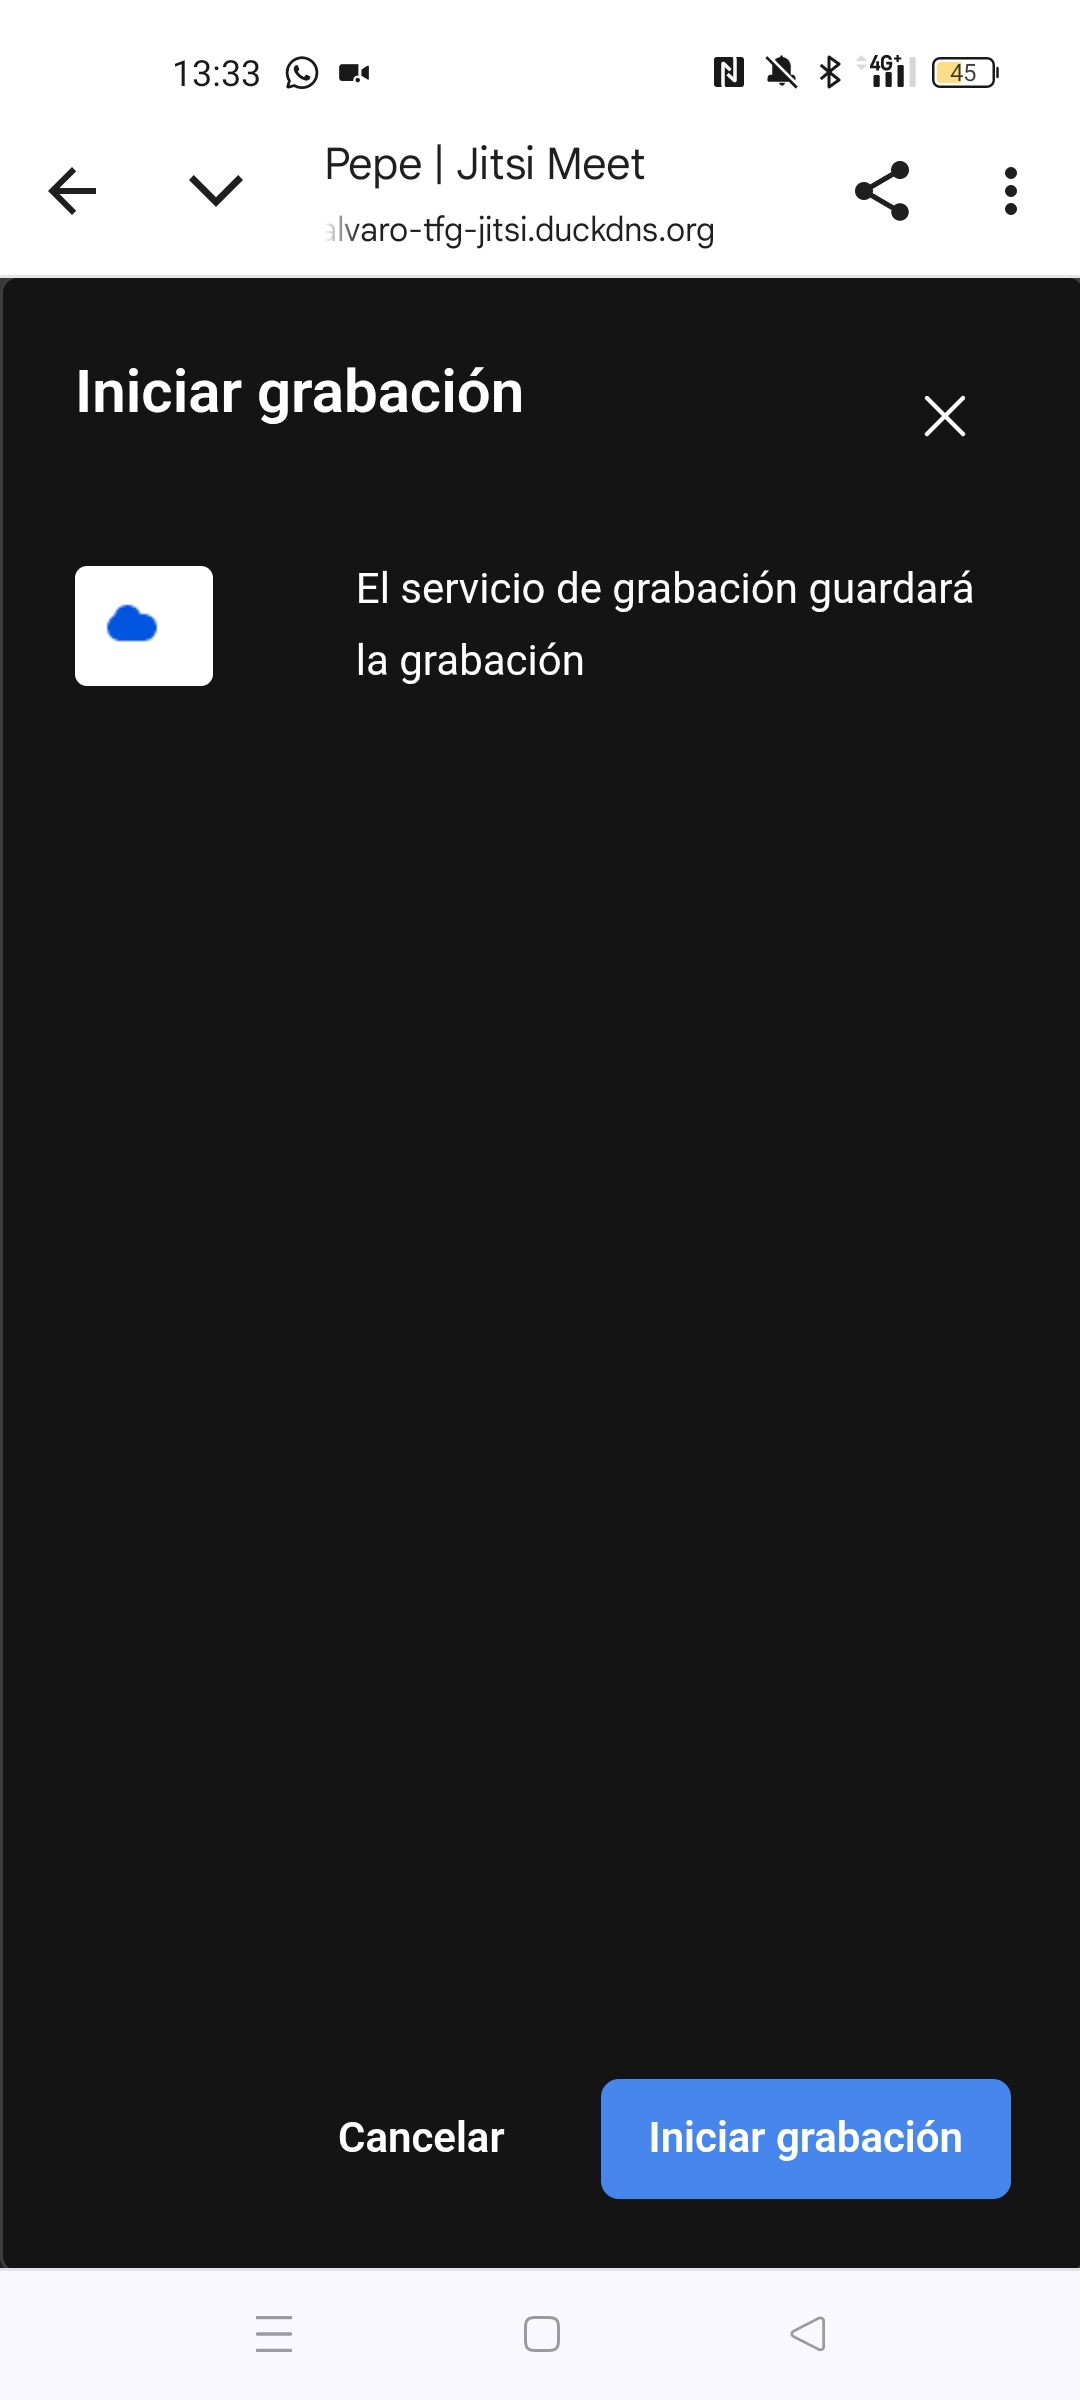
\includegraphics[height=0.6\textheight]{img/iniciargrabacion.jpg}
    \caption{Menú de opciones para iniciar la grabación de la sesión.}
    \label{fig:manual_iniciar_grabacion}
    \end{figure}
    
    \begin{figure}[H]
    \centering
    
\includegraphics[height=0.6\textheight]{img/grabacion.jpg}
    \caption{Indicador visual \textit{REC} que muestra que la sesión se está grabando activamente.}
    \label{fig:manual_grabando}
    \end{figure}
    
    \item \textbf{Detener la grabación:} Para finalizar, el Terapeuta repite el proceso y selecciona "Detener grabación".
\end{enumerate}

\subsection{Verificar el Vídeo Grabado}
Tras detener la grabación, el servicio Jibri tardará unos instantes en procesar y guardar el fichero.
\begin{enumerate}
    \item \textbf{Localizar el fichero:} El archivo MP4 resultante se guardará en el directorio del sistema anfitrión: \\ \texttt{\textasciitilde{}/.jitsi-meet-cfg/jibri/recordings/}.
    \item \textbf{Verificar contenido:} El Administrador puede reproducir este fichero para confirmar que el audio y el vídeo se han grabado correctamente. Este fichero es la entrada para el pipeline de procesamiento.
\end{enumerate}

\begin{figure}[H]
    \centering
    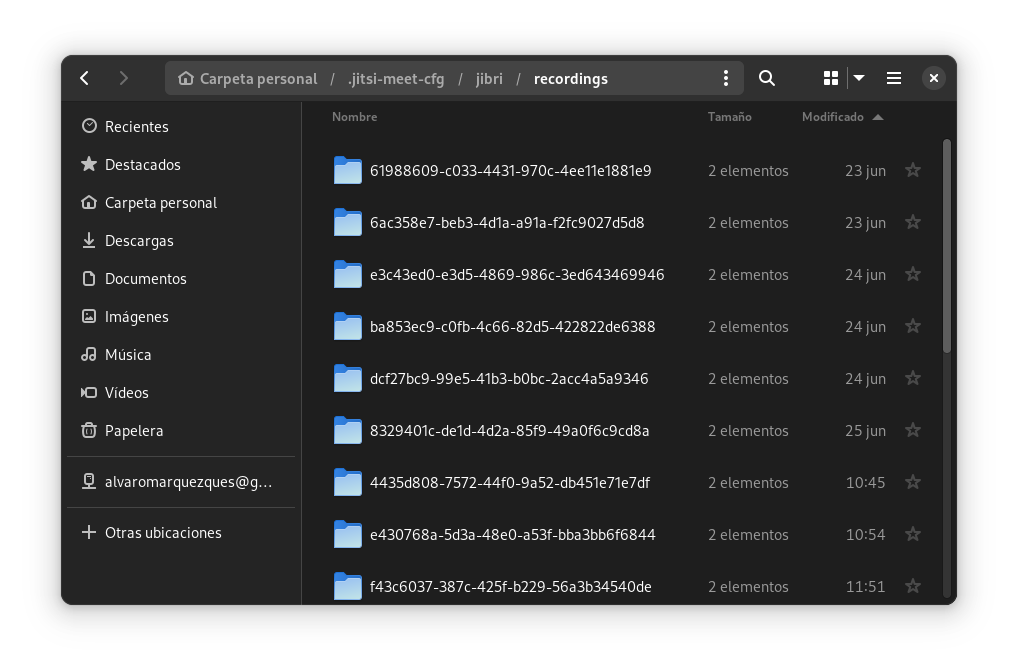
\includegraphics[width=\textwidth]{img/carpetarecordings.png}
    \caption{Ejemplo del directorio de grabaciones de Jibri con el fichero MP4 resultante.}
    \label{fig:manual_carpeta_grabaciones}
\end{figure}

\subsection{Ejecutar y Monitorizar el Procesamiento}
El pipeline de procesamiento está diseñado para ejecutarse de forma automática y continua.
\begin{enumerate}
    \item \textbf{Ejecución automática:} El \textit{script} \texttt{main.py} dentro del contenedor \texttt{python-processor} está constantemente buscando nuevos vídeos en el directorio de entrada.
    \item \textbf{Monitorizar el proceso:} Para ver el progreso en tiempo real, el Administrador puede ejecutar el siguiente comando en la terminal, desde la carpeta \texttt{/src} del proyecto:
    \begin{verbatim}
docker compose logs -f python-processor
    \end{verbatim}
    En la salida se podrán observar mensajes indicando qué vídeo se está procesando.
\end{enumerate}

\begin{figure}[H]
    \centering
    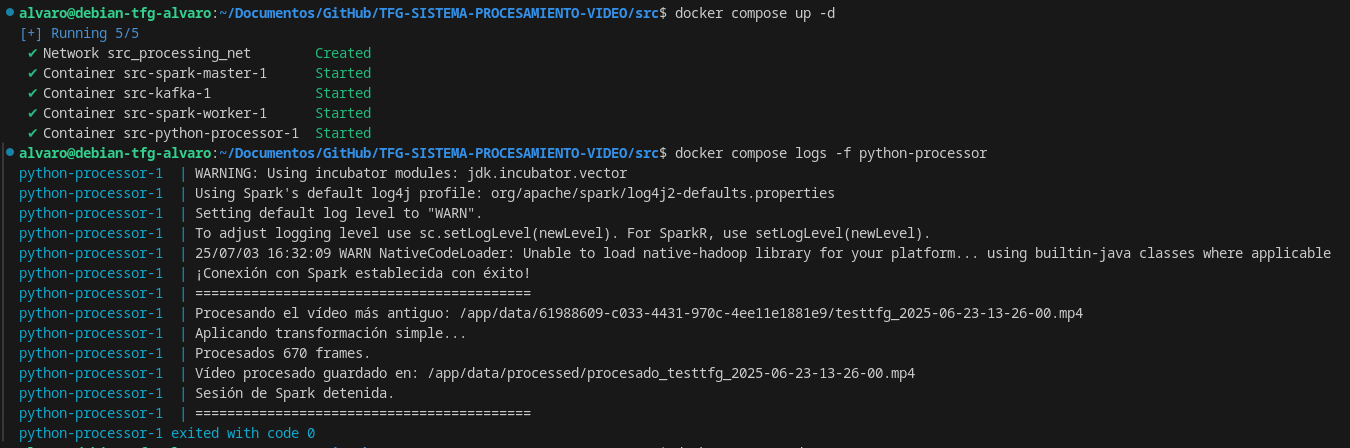
\includegraphics[width=\textwidth]{img/logsfinalpy.png}
    \caption{Monitorización de los logs del procesador Python, confirmando la ejecución del pipeline.}
    \label{fig:manual_logs_procesador}
\end{figure}

\subsection{Acceder al Resultado Final}
Una vez que el \textit{log} indica que el procesamiento ha finalizado, los resultados se pueden encontrar en las siguientes rutas (relativas a la carpeta del proyecto). El vídeo procesado aparecerá en la sub-carpeta /processed y el vídeo original será movido a la sub-carpeta /archived, ambas dentro del directorio donde se guardó originalmente la grabación (por defecto, ~/.jitsi-meet-cfg/jibri/recordings/):
\begin{itemize}
    \item \textbf{Vídeo procesado:} El nuevo vídeo con la transformación aplicada se encontrará en \texttt{/src/data/processed/}.
    \item \textbf{Vídeo original archivado:} El vídeo original que ha sido procesado se moverá a \texttt{/src/data/archived/} para evitar su procesamiento de nuevo.
\end{itemize}

\begin{figure}[H]
    \centering
    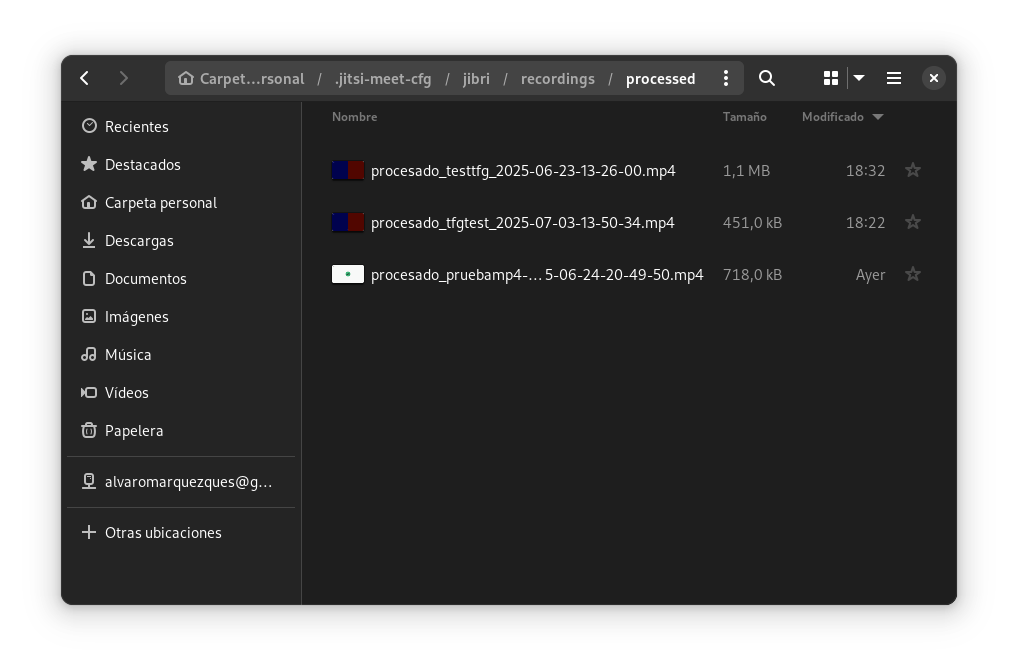
\includegraphics[width=\textwidth]{img/carpetaprocessed.png}
    \caption{Directorio de salida mostrando el vídeo final una vez procesado.}
    \label{fig:manual_carpeta_procesado}
\end{figure}

\section{Resolución de Problemas (FAQ)}
\label{sec:manual_faq}
\begin{itemize}

    \item \textbf{Problema:} No se puede acceder a la instancia de Jitsi desde internet.
    \item \textbf{Causa y Solución:} Verificar que el servicio de DNS dinámico \\ (DuckDNS) está apuntando a la IP pública correcta y que la re-dirección de puertos (80, 443) está bien configurada en el \textit{router}.

    \item \textbf{Problema:} El contenedor \texttt{python-processor} falla al iniciar con un error de conexión a Spark.
    \item \textbf{Causa y Solución:} Esto puede ser una "condición de carrera". El \textit{script} intenta conectar con Spark antes de que el clúster esté completamente listo. El \textit{script} incluye un retardo para mitigar esto, pero si el problema persiste, se puede probar a reiniciar únicamente el contenedor del procesador: \texttt{docker compose restart python-processor}.

    \item \textbf{Problema:} El \textit{log} del contenedor python-processor muestra un error "ModuleNotFoundError" o un conflicto de versiones con NumPy.
    \item \textbf{Causa y Solución:} Esto se debe a una incompatibilidad entre las librerías de Python. Asegúrese de que el fichero \texttt{requirements.txt} del procesador especifica las versiones correctas y compatibles (pyspark==3.5.0, numpy<2.0) y reconstruya la imagen con el comando \texttt{"docker compose up --build"}.

    \item \textbf{Problema:} Al intentar ejecutar un contenedor de Jitsi (especialmente Jibri) aparece un error "s6-mkdir: permission denied" incluso usando sudo.
    \item \textbf{Causa y Solución:} Este es un problema avanzado causado por una incompatibilidad entre el sistema de inicio s6-overlay de la imagen de Docker y el entorno del \textit{host}. La solución implementada en este TFG fue construir una imagen de Jibri personalizada desde un Dockerfile limpio para evitar el conflicto. Consulte la documentación técnica (Apéndice D) para más detalles sobre esta implementación.
    
\end{itemize}